\chapter[The Nature of Differences Between Breeds]{The Nature of Differences Between Breeds (or Races or Species or Other Groups) Averages}
\label{cha:differences-between-group-averages}
\index{Breed differences|(}
\index{Variation!of averages|(}

Averages vary less than the individual items on which they are
based. This happens because the items averaged together are not all
alike and their variations partly cancel each other. The average of a
sample of \textit{n} individuals will differ from the average of the population
from which it came by one \textit{n}th of the sum of the individual deviations
which did not happen to be canceled. If the sample is selected at random,
that difference will be small, especially if the sample is large. The
variance of the averages of such random samples is one nth as large as
the variance of individuals. But, if the sample is selected by some method
which tended more often than not to choose individuals with plus
(or with minus) deviations, those individual deviations will be prevailingly
in the same direction and will not cancel each other completely.
Instead, the sample average will tend to be different from the population
average by an amount determined by the method of selection. In
such a case the variation within the sample will be less than if it had
been selected at random.

As a numerical example we may take annual butterfat production,
for which the standard deviation among cows in Iowa cow testing associations
is not far from 100 pounds. We are not much surprised if we
choose two cows at random and find that their records differ by as much
as 100 pounds. In fact, nearly half of all such pairs would differ by that
much or more. But we would be surprised if the average of two groups
of 10 cows, each selected entirely at random, differed by as much as 100
pounds. We would not expect that to happen oftener than once in
about 20 or 25 such comparisons. If it did happen, we would wonder
whether the two groups really had come from the same population or
whether they had been selected in some biased way which tended to
bring higher records into one group and lower ones into the other. If
the one set had all been selected from one herd and the other set had all
come from another herd, we would not be so surprised by that big a
difference, since good or poor management or breeding in either herd
would tend to shove all the records from that herd up or all down
together. In choosing only two herds at random it might easily happen
that we would get one herd with poor management and another with
good management; while, if each record came from a different herd, it
is not at all likely that the IO in one set would all come from well-managed
or well-bred herds and the IO in the other set would all come from
poor herds, unless there was some difference in the method of choosing
the records for each set.

\begin{figure}
	\centering
    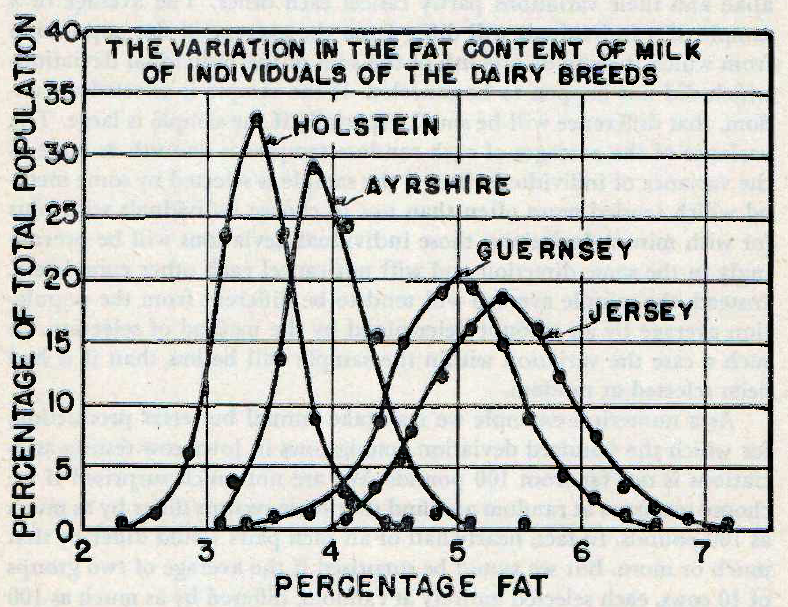
\includegraphics[width=\textwidth]{Figure_10.png}
    \caption{Distributions of individual cows in four dairy breeds according to the
			 percentage of butterfat in their milk. The breeds overlap, but the differences between
			 their averages are real. (Adapted from Bul. 365 of the Mo. Agr. Exp. Station.)}
    \label{fig:Lush_Figure_10}
\end{figure}

Because averages are less variable, it is often possible to be sure that
there is a real difference between two groups which have averages not
very different and in which the individuals vary so widely that the two
groups overlap in much of their range. This is the general situation for
most breed differences, especially for differences in economically important
and physiologically complex characteristics like milk production,
fertility, size or shape of muscular parts, etc. Figure~\ref{fig:Lush_Figure_10} shows this for
percentage of fat in the milk of four breeds of dairy cattle. For some
characteristics, notably color or details of bone dimensions or conformation,
there may be no overlapping at all between breeds. Figure~\ref{fig:Lush_Figure_11}
illustrates graphically the relation between individual differences and
group differences. The fairly common saying, ``There is more difference
within breeds than there is between breeds,'' is often true in the sense
that the difference between the breed averages is small compared with
many of the differences between individuals which belong to the same
breed. This saying is quite misleading, however, if it is interpreted to
mean that the differences between breeds are not real after all. Group
differences of the same kind as are illustrated in Figure~\ref{fig:Lush_Figure_11} often prevail
between races and may prevail between families or other groups
within a breed.

\begin{figure}
	\centering
    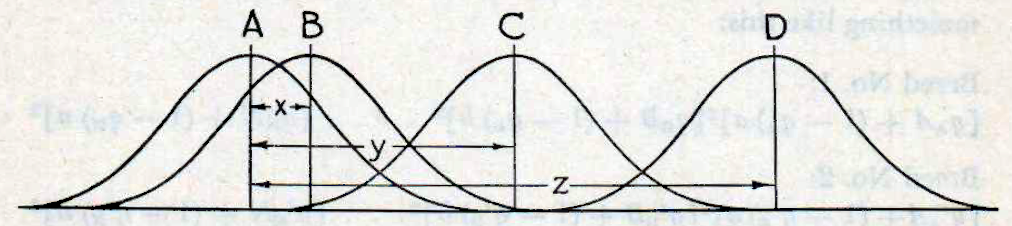
\includegraphics[width=\textwidth]{Figure_11.png}
    \caption{Overlapping frequency curves showing the nature of differences between
			population averages and differences between individuals. \textit{x} is
			the difference between the averages of populations \textit{A} and
			\textit{B}, which overlap in most of their ranges. \textit{y} is the
			difference between the averages of populations \textit{A} and
			\textit{C}, which overlap only a little. \textit{z} is the difference
			between the averages of populations \textit{A} and \textit{D}, which do
			not overlap at all. If two individuals are chosen at random from one
			population. The difference between those two will be larger than
			\textit{x} in far more than half of such pairs and in a few pairs will
			be larger than \textit{y}.}
    \label{fig:Lush_Figure_11}
\end{figure}

It is to be expected that breeds which have been kept separate from
each other in their ancestry for many generations will usually have
drifted apart in many of their characteristics on account of the sampling
variations of Mendelian inheritance in small populations, or will have
been drawn apart by selection which has not been equally successful in
both breeds or has not been directed toward exactly the same ideals.
Breed differences may often be so small that they are economically
unimportant, especially if the breeds have been selected toward almost
the same ideals; yet it would be a remarkable coincidence if the breed
averages were exactly the same for any characteristic. Even where two
breeds have been selected toward the same ideal and their phenotypic
averages are almost the same, the sets of genes by which that phenotype
is produced are likely to have become qualitatively different if the two
breeds have been kept entirely from any crossing with each other for
tens of generations.
\index{Variation!of averages|)}

\index{Homozygosis}
The genetic basis of differences between breeds may be of two kinds.
In the first place, one breed may be homozygous for one gene and
another breed may be homozygous for an allel of that gene. If that were
true for all genes\\index{Variation!as affected by gene numbers|(}\index{Zygotic ratios|(}, we could write the Mendelian formulas of two breeds
as follows:

\begin{table}[htbp]
	\centering
	\begin{tabular}{L{2.5cm}L{2.5cm}L{2.5cm}}
		Breed No. 1		& \textit{AABBccddEE}	&	\textit{NN}	\\
		Breed No. 2		& \textit{aabbCCddEE}	&	\textit{nn}	\\
	\end{tabular}
\end{table}

\noindent
This would indicate that the two breeds are homozygous for different
genes in the series for \textit{A}, for \textit{B}, £or \textit{C} and
for \textit{N}, but are alike in the series for \textit{d} and for
\textit{E}. This conception of breed differences appears to have
been rather widely held by those who discussed the possible practical
applications of Mendelism in the early years of genetics, but it is
expressed less frequently now, as the evidence accumulates that few
genes are homozygous in all members of the breed. The other kind of
genetic situation which may be the basis for distinct breed differences is
that a pair of genes is not entirely homozygous in either breed but the
proportion of one gene to its allel may be widely different in the two
breeds. \index{Gene frequency|(}The Mendelian formulas for the two breeds could be written
something like this:

\begin{table}[htbp]
	\centering
	\begin{tabular}{l}
		Breed No. 1		\\
		$[q_AA + (1-q_A)a]^2[q_BB + (1-q_B)b]^2 \cdots [q_NN + (1-q_N)n]^2$ \\
		\\
		Breed No. 2 \\
		$[q'_AA + (1-q'_A)a]^2[q'_BB + (1-q'_B)b]^2 \cdots [q'_NN + (1-q'_N)n]^2$ \\
	\end{tabular}
\end{table}

\noindent
The blood groups in the Guernsey and Holstein-Friesian breeds of cattle
are a good example of this very situation (\textit{Jour. Ani. Sci.} 3:315--321.
1944). In an extreme case of this sort, such as is illustrated in Figure 12,
two breeds might be alike in the sense that every kind of gene which
exists in the one also exists in the other, and yet be distinctly different
outwardly and in average genotype. Genetic differences of both kinds
probably exist between most breeds. Really, the first kind of difference
is only an extreme limit of the second where \textit{q} = 1.0 in one breed and
is zero in the other.

A complete description of a breed involves not only a statement of the genes
for which it is homozygous and different from other breeds but also a statement
of the frequencies in it of genes for which it is not homozygous and which other
breeds may also possess in larger or smaller frequencies. Thus, a complete
description of a black breed of cattle may contain, besides the statement that
the ``type'' (the most frequent kind) is black, the statement that in this breed
the frequency of gene \textit{B} is .93 and of \textit{b} is .07. Perhaps in
another black breed the frequency of \textit{B} may be .97 or perhaps only .80,
while in a breed like the Shorthorn, where solid black is unknown, the frequency
of \textit{B} is .00. Perhaps other alleles in this series may yet be found.
For example, the genetic explanation of the black pigment present in fawn or
brindle breeds or of such dark pigment as occasionally appears around the eyes
or muzzles of Shorthorns is still uncertain. If such other alleles are found, a
complete description of some other breed may include the statement that in it the
frequency of \textit{B} is .40, of $B_1$ is .45, and of \textit{b} is .15. Naturally
it will be difficult to get such complete information except for a few genes which
individually have conspicuous effects. For a long time to come it is likely that
the practical description of a breed will consist mainly of its averages, or
``type'' in traits which do not lend themselves readily to numerical averaging, with
a few sketchy semi-quantitative comments about its variability in those features.
\index{Gene frequency|)}

\begin{figure}
	\centering
    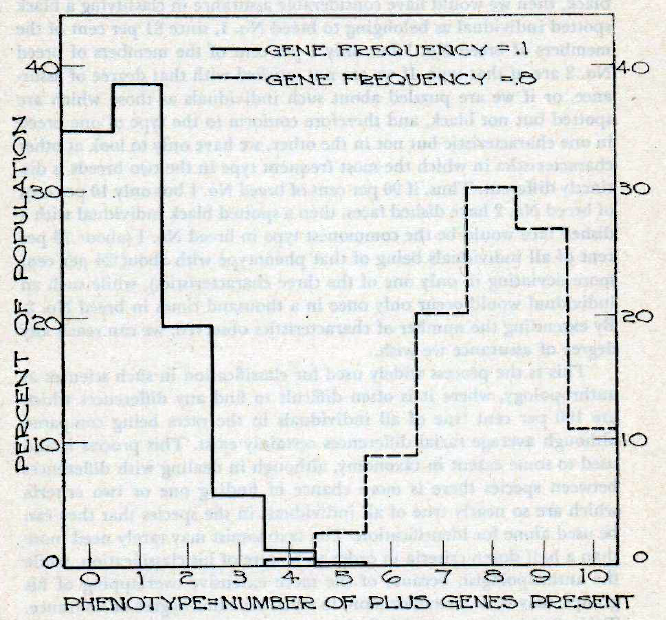
\includegraphics[width=\textwidth]{Figure_12.png}
    \caption{The distribution of genotypes expected in two random breeding populations
			 each of which is heterozygous for five pairs of genes with equal effects. The
			 genes lack dominance and combine their effects additively. In one population the
			 frequency of the plus gene in each of the five pairs is .1, while in the other it is .8.
			 This will illustrate how two breeds could both have exactly the same kinds of genes
			 and yet overlap so little that there would be practically no mistakes in classifying
			 individuals.}
    \label{fig:Lush_Figure_12}
\end{figure}

Two breeds may overlap in every observable characteristic, and yet
it may be possible to identify with certainty the breed to which every
individual belongs. If 90 per cent of the individuals in breed No. 1 but
only 10 per cent of those in breed No. 2 are spotted, we cannot with
much assurance classify the breed of an individual by examining it for
spotting alone. There are too many exceptions to the ``type.'' But if 90
per cent of the individuals in breed No. 1 are black in their colored
areas, while only 10 per cent of the individuals in breed No. 2 are
black, then we would have considerable assurance in classifying a black
spotted individual as belonging to breed No. l, since 81 per cent of the
members of breed No. 1 but only 1 per cent of the members of breed
No. 2 are of that type. If we are not satisfied with that degree of assurance,
or if we are puzzled about such individuals as those which are
spotted but not black, and therefore conform to the type of one breed
in one characteristic but not in the other, we have only to look at other
characteristics in which the most frequent type in the two breeds is distinctly
different. Thus, if 90 per cent of breed No. 1 but only 10 per cent
of breed No. 2 have dished faces, then a spotted black individual with a
dished face would be the commonest type in breed No. 1 (about 73 per
cent of all individuals being of that phenotype with about 24 per cent
more deviating in only one of the three characteristics), while such an
individual would occur only once in a thousand times in breed No. 2.
By extending the number of characteristics observed, we can reach any
degree of assurance we wish.

This is the process widely used for classification in such sciences as
anthropology, where it is often difficult to find any differences which
are 100 per cent true of all individuals in the races being compared
although average racial differences certainly exist. This process is also
used to some extent in taxonomy, although in dealing with differences
between species there is more chance of finding one or two criteria
which are so nearly true of all individuals in the species that they can
be used alone for identification. The taxonomist may rarely need more
than a half dozen criteria in order to be sure of his classification, while
the anthropologist, because of the more extensive overlapping of his
groups, may need a score or more to reach the same degree of assurance.
Table~\ref{tbl:Lush_Table_9} shows in some detail the average number of
\index{Deviations from type|(} deviations from
``type'' which may be expected per individual in a population where
\textit{n} independent characteristics are being examined and in each of those
characteristics \textit{t} is the fraction of individuals which deviate from type.
The average number of deviations expected in an individual is \textit{nt}. The
figures which follow the $\pm$ signs are standard deviations computed by
the formula, $\sigma = \sqrt{nt(1 - t)}$, which must be interpreted with
reservation on account of the distinct skewness of the distribution where \textit{t} is
far from .5. The standard deviations show that, when the average number
of deviations from type is large, there may be no individuals which
are exactly like the ``type.'' For example, when \textit{n} = 20 and \textit{t} = .40, the
average individual will deviate from ``type'' in 8 respects, only about
one-eighth of them will deviate from type in as few as 5 respects, only 1
in 20 in as few as 4 respects. Less than I in 27,000 will conform exactly
to type in all 20 respects. In this sense it may be true that in finite populations
there is \textit{no such thing as an average individual}, but that does not
impair the usefulness of the average for describing the group. The
description of the group will be more complete if something is also
stated about the variation to be expected in each characteristic.

\begin{table}
	\centering
	\caption{\textsc{Average Number of Characteristics per Individual Expected to Deviate From
			 the ``Type'' of the Group Where} \textit{n} \textsc{Characteristics are Observed
			 and} \textit{t} \textsc{is the Fraction of Individuals Which Deviate From Type in
			 Each Respect}}
	\label{tbl:Lush_Table_9}
	\begin{tabular}{L{2cm}|C{3cm}|C{3cm}|C{3cm}}
		\hline
		\hline
					& \multicolumn{3}{c}{\textit{n}} \\
		\cline{2-4}
		\textit{t}	& 5				& 10			& 20 \\
		.01			& .05 $\pm$ .2	& .1 $\pm$ .3	& .2 $]pm$ .4 \\
		.05			& .25 $\pm$ .5	& .5 $\pm$ .7	& 1.0 $]pm$ 1.0 \\
		.20			& 1.0 $\pm$ .9	& 2.0 $\pm$ 1.3	& 4.0 $]pm$ 1.8 \\
		.40			& 2.0 $\pm$ 1.1	& 4.0 $\pm$ 1.5	& 8.0 $]pm$ 2.2 \\
		\hline
	\end{tabular}
\end{table}
\index{Variation!as affected by gene numbers|)}

The same principles used in classifying individuals may be extended
to the classification of groups wherever it appears likely that the groups
are random samples or systematic samples selected fairly. One will often
see a Jersey cow which is broken-colored and in that respect is more like
the Guernsey breed than the Jersey; but one will almost never see a
herd of Jerseys which are all broken-colored, although that is the usual
description of a herd of Guernseys. A broken-colored Jersey without any
black pigment, although rare, sometimes occurs and might be mistaken
for a Guernsey if color alone were considered. One would never see a
herd of Jerseys which were all broken-colored and free from black pigment.
\index{Deviations from type|)}
\index{Zygotic ratios|)}

\section*{DIFFERENCES BETWEEN SPECIES}
\index{Species!nature of differences between|(}

A species is a more or less continuous and interbreeding group as
actually found in nature. To practical taxonomists discontinuity
between two groups is the criterion of whether or not they are really
different species. This leaves room in some cases for disagreement as to
justify calling the population one species. Two groups of similar individuals
which are not connected by any intermediates are universally
recognized as valid, or ``good,'' species. On the other hand, two groups
of individuals may be widely different in the averages of many of their
traits and yet, if they are connected by a complete series of intermediate
individuals, most practical taxonomists would regard them as really one
species with a tendency to exist in several varied forms or subspecies.
This situation is much the same as might be encountered in deciding in
a mountainous region whether one were describing two distinct mountain
ranges or one group of mountains. If there were a broad and deep
valley separating the mountains, everyone would agree that they were
two distinct ranges. If the intervening space were occupied by a group
of large hills or low mountains, irregular in outline, some might still
wish to call them two mountain ranges, but others would think the
whole group should be called by one name. The fact that there is sometimes
room for argument about whether a group is one species with two
subspecies or is two separate species does not contradict the fact that
there are such things as species groupings in nature, any more than the
reality of mountains is contradicted by a dispute as to whether some
particular elevation is one mountain with two peaks or is two separate
mountains.

Besides being a matter of practical convenience, the taxonomic system
attempts to describe the general fact that the existing plants and
animals are not scattered uniformly all through the infinite field of possible
combinations of form and function and appearance and behavior,
but are definitely and irregularly clumped around certain types, most of
which are separated from the nearest similar types by a considerable
void of conceivable intergrades which do not occur. This is like the distribution
of matter in astronomical space, which is highly discontinuous
and irregular with definite clumps, like planets, stars, etc., which
are themselves clustered in irregular groups like solar systems, constellations,
nebulae, etc. The interesting cases about which there is dispute as
to species classification are those where a few of those conceivable intergrades
actually do occur and form a nearly continuous connection
between two nearby clumps, or where the clump itself seems to have
two or more separate centers of density around which the existing forms
are clustered more closely than elsewhere in the clump. Quite conceivably
these may be centers of incipient formation of new species, but in
particular cases they may be still so close together and connected by so
many intergrades that there can be no reasonable argument for elevating
them to specific rank.

\index{Evolution|(}
The early taxonomists often had an exaggerated idea of the supposed
uniformity of wild species. Traces of that idea still linger in biological
literature. Much of this doubtless comes from a more or less
unconscious deference to the opinions of Linnaeus (Carl von Linn\'{e},
1707--1778), the Swedish naturalist who devised the present binomial
system of naming plant and animal species.\footnote{For example, on page 128 of
\textit{Biology and Its Makers}, by Locy, we read: ``Ray
had spoken of the variability of species but Linnaeus in his earlier publications
declared that they were constant and invariable''; and on page 129: ``While Linnaeus
first pronounced upon the fixity of species, it is interesting to note that his extended
observations upon nature led him to see that variation among animals and plants is
common and extensive, and accordingly in later editions of his \textit{Systema Naturae} we
find him receding from the position that species are fixed and constant. Nevertheless,
it was owing to his influence more than to that of any other writer of the period,
that the dogma of fixity of species was established.''} Today it is recognized with
increasing clarity that the more one studies a wild species, the more differences
he finds among the individuals composing it. If he makes several
different collections of individuals of the same species, each collection
having been trapped in a different locality, he will usually find each
collection different enough from the others that if he were to see another
\textit{collection} made from one of those same localities he would be able to
identify the locality from which it came, although he would not be able
surely to identify the locality of each animal presented to him singly. In
short, even the ``good'' species differ from locality to locality, particularly
among animals which do not travel far.\footnote{Sumner, Francis B. 1934.
``Taxonomic Distinctions Viewed in the Light of Genetics.'' Amer. Nat., 68:137--149.}

The definition of a species has a peculiar relation to the idea of special
creation. Linnaeus believed firmly in the special creation of each
individual species, as did most other people of his time. The belief in
special creation necessitated a belief that there was a real nature-made
difference between species. Hence, there would be some fundamental
valid distinction between species which, if one could only discover it,
would serve as an accurate touchstone for deciding in accordance with
natural laws what was and what was not a true species. Linnaeus, as
well as all contemporary and succeeding naturalists, recognized that
orders, genera, etc., were divisions made by man, as a matter of convenience,
for classifying together organisms which had certain general
resemblances. They regarded subspecies, varieties, breeds and such divisions
of a species as matters of convenience or as the result of man's
handiwork and therefore outside the scheme of nature. This insistence
that the difference between species is a fundamental one on an entirely
different basis from other differences in classification explains the intensity
of many arguments about what constituted a real species in particular
cases. The acceptance of the idea of organic evolution carries with it
the consequence that species differences are no less and no more manmade
than differences between genera or orders. The difference
between species is taken out of a special category and becomes only a
matter of degree in the general system of classification.

The modern genetic idea of species differences is that they are similar
in kind to the breed differences explained above but are much more
extreme, so that discontinuity is an essential part of the species definition.
Also, in most cases, the two sets of genes are so different that they
will not work together harmoniously in producing their physiological
effects. Hence, crosses between species\index{Species!crosses} are usually (but not always)
impossible or, if possible, are usually sterile. Since inheritance is in duplicate,
it will sometimes happen that the first cross hybrids which have a
complete but single set of the genes from each parent can function all
right in their own physiology (as is the case with the mule\index{Mules}) but cannot
reproduce because the genes from the different kinds of parents are so
unlike that they will not pair properly enough for the reduction division
to take place. Even if reduction does occur, the resulting sample of
genes will rarely have all that are necessary for harmonious functioning.
It is somewhat as if one were to try to make a workable automobile
from two different kinds by fastening together cylinders from one, pistons
from the other, a fuel pump from the first, a carburetor from the
second, cam shaft from one, distributor from the other, etc. If the two
makes of automobiles were very different, it would be the rarest kind of
a coincidence if such an automobile would run at all.

Discontinuity of ancestry between breeds is a fairly recent thing and
does not go back much farther than the beginnings of the herdbooks in
some cases. Separateness of ancestry between species is a vastly older
thing, going far back into geologic time in most cases. Whenever two
subgroups of a single group cease to interbreed, their genetic averages
tend to become different, either through the random drift of gene frequencies
in the sampling which takes place each generation during the
reduction division, or because the direct effects of selection may be different
if the subgroups live in different regions or otherwise occupy
different ecological niches. Both processes can be supplemented by
mutations which may not be the same in both groups. Once discontinuity
of interbreeding is established, it is easy to see how two subgroups of
a species not only might but must in geologic time drift apart so far that
they could not cross.

The most puzzling problem in the origin of species is how the discontinuity
of interbreeding first arose in each case of a dividing species. Natural
selection differently directed in different regions might have made portions
of a species become unlike; but, unless they were so distinctly separated
that there was almost no interbreeding between the two groups, it seems likely
that crosses between them would usually prevent that from going far enough to
form two separate species. Discontinuity of interbreeding might have been brought
about by geographic isolation; but, as nearly as we can interpret the geologic
record, changes of sufficient magnitude to bring that about seem to have been too
slow to provide enough isolation to account for the facts of evolution.
Irregularities in the chromosome mechanism, such as polyploidy or frequent and
extensive inversions, might have brought about discontinuity of interbreeding even
without geographic isolation. These probably did play a considerable part in the
evolution of plants, but it is generally thought that their effect on animals must
have been much less important, both because the chromosome numbers among so many
of the modern mammals are so similar and because self-fertilization and asexual
reproduction are not possible in higher animals. One with a chromosome abnormality
probably could not find a mate like itself, and it or its offspring from normal
mates would usually be sterile. Assortive mating may have played a part, although
most students of the subject now think the importance of that was overestimated by
Darwin in his writings on sexual selection. Inbreeding is a powerful force for
differentiation of groups, but there is uncertainty about how much of that
actually occurs in nature.\footnote{For a general survey of the possibilities in
that, see: Wright, Sewall. 1940. ``Breeding Structure of Populations in Relation
to Speciation.'' \textit{Amer. Nat.} 74:232--48. See also the chapter on isolating
mechanisms in T. Dobzhansky's \textit{Genetics and the Origin of Species}. 1941.
Columbia University Press.} Perhaps all these processes played a part, varying in
importance in different cases. The subject is full of interest to the philosophy
of biology but contributes little to the routine practice of the animal breeder
since he can establish discontinuity in his wn breeding operations in whatever
way he wishes.
\index{Evolution|)}
\index{Species!nature of differences between|)}

\section*{SUMMARY}

\begin{enumerate}
\item Because of the lessened variability of averages it is often possible
to distinguish breeds (or other groups) whose averages are not very far
apart even though the individuals within each breed vary widely and
the breeds overlap.
\item Breeds may differ in one's having a gene which is entirely absent
from the other, but more commonly they differ in the frequencies of
genes which are present in both.
\item By considering a sufficient number of characteristics in which
the averages of two breeds are different, it is possible to identify with
any desired degree of certainty the members of each, even though both
breeds overlap each other's range in all those characteristics.
\item Differences between species are thought to have the same genetic
basis as the differences between breeds but are so much more extreme
that crosses between species are usually sterile, if possible at all .
\item A species is a more or less continuous and interbreeding group as
actually found in nature. To the practical taxonomist the discontinuity
rather than the magnitude of the differences between species is the most
satisfactory criterion of whether they are really two species or a single
variable one.
\item The most puzzling problem in the origin of species is how the
discontinuity of interbreeding first arose in each case. Several explanations
are possible, but it is not certain which of them has been the main
explanation in most cases.
\end{enumerate}
\index{Breed differences|)}